\documentclass[12pt,a4paper]{article}

\usepackage[T1]{fontenc}
\usepackage[utf8]{inputenc}
\usepackage[spanish,provide=*]{babel}
\usepackage[margin=2.5cm, top=2.4cm, bottom=2.6cm]{geometry}
\usepackage{graphicx}
\usepackage{fancyhdr}
\usepackage{enumitem}
\usepackage{listings}
\usepackage{float}
\usepackage{tikz}
\usepackage[font=small, labelfont=bf, skip=6pt]{caption}

\graphicspath{{includes/}}

\lstset{
    basicstyle=\ttfamily\small,
    breaklines=true,
    columns=fullflexible,
    keepspaces=true,
    showstringspaces=false,
    tabsize=4,
    aboveskip=8pt,
    belowskip=8pt
}

\tikzset{
    caja/.style={draw, align=center, inner sep=7pt, font=\small},
    flecha/.style={->, thick}
}

\pagestyle{fancy}
\fancyhf{}
\setlength{\headheight}{14pt}
\rhead{\small Programación Concurrente: TP2}
\rfoot{\thepage}
\renewcommand{\headrulewidth}{0.3pt}

\setlist[enumerate]{itemsep=0.45em, topsep=0.5em, leftmargin=1.4em}
\setlist[itemize]{itemsep=0.25em, topsep=0.4em}

\begin{document}

\begin{titlepage}
\thispagestyle{empty}
\centering
\vspace*{1.6cm}

\includegraphics[width=2.8cm]{fiuba}

\vspace{0.9cm}
{\small\scshape Universidad de Buenos Aires}\\[0.2em]
{\small\scshape Facultad de Ingeniería}

\vspace{2.1cm}
{\large Programación Concurrente}\\[0.25em]
{\small Curso Musso, 2\textsuperscript{do} cuatrimestre 2026}

\vspace{1.15cm}
{\LARGE Motor Distribuido de Reservas y Pagos}\\[0.45em]
{\large Trabajo Práctico Nº 2}

\vspace{1.5cm}
\begin{tabular}{@{}p{7.2cm} r@{}}
Basile, Joaquín Ezequiel & 111687 \\[0.35em]
Binker, Alejandro & 107056 \\[0.35em]
Giovanettoni, Máximo & 110303 \\[0.35em]
Verne, Bruno & 112176 \\
\end{tabular}

\vfill
\end{titlepage}

El trabajo es el núcleo de una venta de entradas. La cuenta de cada usuario y los asientos viven en actores distintos: el estado queda en el hilo de cada uno, y una compra se resuelve mandando mensajes.

\section{Modelos de concurrencia y actores}

La plata de un usuario y las entradas no comparten memoria. Cada una es un actor: un hilo con su estado adentro y un buzón. El código está en el módulo \texttt{actores} del crate \texttt{tp2\_reservas}. Esta parte se corre con \texttt{cargo run -- parte1}.

El armado es el de la actividad de transferencias. Se abre un canal \texttt{mpsc}, el \texttt{Receiver} se mueve al hilo y la función devuelve el \texttt{Sender}. Esa es la dirección del actor. El estado no está en un struct compartido: es un \texttt{let mut} de ese hilo.

\subsection{CuentaUsuario}

El saldo arranca en el valor que recibe \texttt{crear\_actor\_cuenta}. El bucle lee el buzón de a un mensaje.

\texttt{ConfirmarDebito} trae el monto y un canal de respuesta. Si el saldo alcanza, lo descuenta y contesta \texttt{Ok}. Si no, contesta \texttt{FondosInsuficientes} y no lo toca. \texttt{ConsultarSaldo} también trae canal de respuesta: devuelve el número actual. Sin esa respuesta el que preguntó no tendría cómo enterarse, porque el saldo no se puede leer desde afuera.

\begin{lstlisting}
for msg in rx {
    match msg {
        MensajeCuenta::ConfirmarDebito { monto, canal_respuesta } => {
            if saldo >= monto {
                saldo -= monto;
                let _ = canal_respuesta.send(RespuestaDebito::Ok);
            } else {
                let _ = canal_respuesta.send(
                    RespuestaDebito::FondosInsuficientes,
                );
            }
        }
        MensajeCuenta::ConsultarSaldo { canal_respuesta } => {
            let _ = canal_respuesta.send(saldo);
        }
    }
}
\end{lstlisting}

\subsection{InventarioEntradas}

\texttt{crear\_actor\_inventario} guarda cuántas entradas quedan. \texttt{SolicitarReserva} resta una si queda alguna y contesta \texttt{Ok}. Si no queda ninguna, contesta \texttt{Agotado}. Para leer el contador está \texttt{ConsultarDisponibles}.

Dos hilos no miran ese contador a la vez. El primero que el actor atiende, si había una entrada, se la lleva. El siguiente ya ve el contador descontado.

\subsection{Data races}

El saldo es una variable local del hilo de la cuenta. Ningún otro hilo tiene una referencia. Para cambiarlo hay que mandar un mensaje: el \texttt{send} le pasa el valor al receptor y el emisor deja de tenerlo.

El \texttt{for} toma un mensaje, termina el \texttt{match} y recién ahí toma el siguiente. Dos débitos no se mezclan en la lectura y la escritura. El segundo ve el saldo que dejó el primero. Con 50 y dos pedidos de 30, uno descuenta. El otro recibe \texttt{FondosInsuficientes}. Quién entra primero depende del orden de la cola. El saldo que queda es el de una de esas dos operaciones.

En el contador del almacén, dos hilos leían la misma palabra, le sumaban uno y escribían. Esas instrucciones se intercalaban y el contador podía quedar en 1 habiendo dos incrementos. Acá esa mezcla no tiene dónde ocurrir: la palabra la escribe un solo hilo. Por eso la cuenta no lleva un lock. Lo mismo pasa con el contador de entradas.

Lo que sí depende del orden es quién se queda con la última entrada. Veinte hilos pueden mandar \texttt{SolicitarReserva} juntos. El inventario los atiende de a uno. Uno solo recibe \texttt{Ok}. Hay contención, y el ganador no está fijo de antemano. No hay dos escrituras a la vez sobre el contador.

El compilador cierra la otra puerta. La variable vive en el closure con el que se lanza el hilo. Otro hilo no puede pedirla prestada para mutarla.

\subsection{Cincuenta mil conexiones}

Esto es el servidor que acepta las conexiones HTTP, no estos actores. Una cuenta es un hilo que vive mientras corre el proceso. Cincuenta mil conexiones son cincuenta mil clientes esperando en un socket.

Un hilo del sistema por conexión reserva su stack. En clase tomamos unos 2~MB por hilo: 10.000 conexiones ya eran del orden de 20~GB, y la mayor parte del tiempo esos hilos están bloqueados en la red. Con 50.000, solo los stacks ocupan unos 100~GB. El planificador del kernel cambia de contexto entre hilos que no tienen nada que calcular.

Con async/await cada conexión es una tarea. El \texttt{async fn} queda como un \texttt{Future}: una máquina de estados. En el \texttt{.await}, si el socket no está listo, la tarea suelta el hilo y ese hilo atiende otra. Tokio reparte las tareas listas sobre un pool chico de hilos de sistema. Un reactor las despierta cuando el sistema operativo avisa que el socket tiene datos. Las 50.000 conexiones son 50.000 estados chicos sobre esos pocos hilos.

\subsection{Pruebas}

\texttt{debitos\_concurrentes\_no\_sobregiran} lanza 50 hilos que piden 30 sobre un saldo de 1000. Es la pregunta de la clase: muchos hilos le escriben al mismo actor a la vez. Entran 33 débitos, que son 990, y \texttt{ConsultarSaldo} devuelve 10. Si dos débitos se pisaran sobre la misma palabra, esa cuenta no cerraría.

\texttt{debito\_sin\_fondos\_no\_toca\_el\_saldo} pide 40 con un saldo de 30. La respuesta es \texttt{FondosInsuficientes} y la consulta sigue en 30.

\texttt{un\_solo\_hilo\_se\_queda\_con\_la\_ultima\_entrada} lanza 20 hilos contra una sola entrada. Una respuesta es \texttt{Ok}, las otras \texttt{Agotado}, y el contador queda en 0.

Corrimos \texttt{cargo test --lib actores}. Las tres pasan. \texttt{cargo run -- parte1} imprime los mismos 33 y saldo 10, y una reserva sobre la única entrada.

\section{Modelado formal con Redes de Petri}

Para analizar el protocolo 2PC simplificado se modela una única
transacción con un coordinador y un participante. En la Figura
\ref{fig:red-petri-2pc} se muestran los lugares como círculos, los mensajes
pendientes como lugares intermedios y las acciones como transiciones
rectangulares.

\begin{figure}[H]
    \centering
    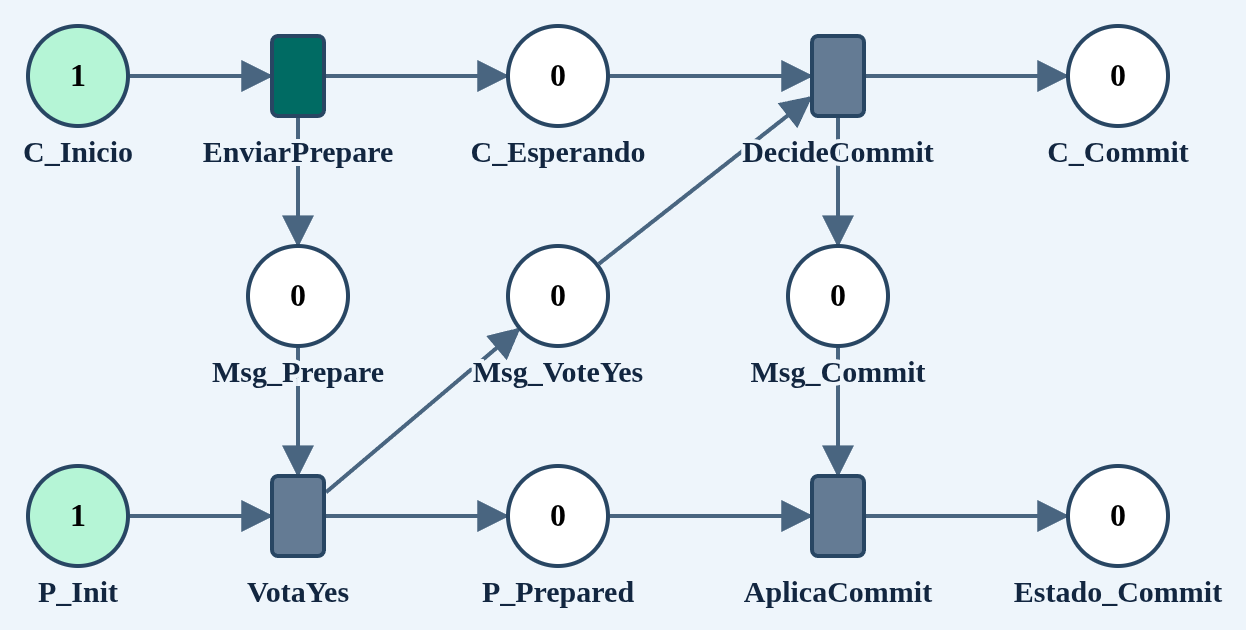
\includegraphics[width=\textwidth]{../diagrama_petri_2pc.png}
    \caption{Red de Petri del protocolo 2PC con un participante.}
    \label{fig:red-petri-2pc}
\end{figure}

\subsection{Lugares y transiciones}

Los lugares principales de la red son:

\begin{itemize}
    \item \texttt{Coordinador\_Inicio}, \texttt{Coordinador\_Esperando\_Votos},
    \texttt{Coordinador\_Commit}, \texttt{Coordinador\_Rollback} y
    \texttt{Coordinador\_Caido}, que representan el estado del coordinador.
    \item \texttt{Participante\_Init}, \texttt{Participante\_Prepared},
    \texttt{Estado\_Commit} y \texttt{Estado\_Rollback}, que representan el
    estado del participante.
    \item \texttt{Msg\_Prepare}, \texttt{Msg\_VoteYes},
    \texttt{Msg\_VoteNo}, \texttt{Msg\_Commit} y
    \texttt{Msg\_Rollback}, que representan mensajes enviados pero todavía no
    consumidos.
\end{itemize}

La marcación inicial tiene un token en
\texttt{Coordinador\_Inicio} y otro en \texttt{Participante\_Init}. La
ejecución exitosa queda descrita por la siguiente secuencia:

\begin{enumerate}
    \item \texttt{EnviarPrepare} mueve el token del coordinador a
    \texttt{Coordinador\_Esperando\_Votos} y genera un token en
    \texttt{Msg\_Prepare}.
    \item \texttt{VotaYes} consume \texttt{Msg\_Prepare} y el token de
    \texttt{Participante\_Init}; deja al participante en
    \texttt{Participante\_Prepared} y genera \texttt{Msg\_VoteYes}.
    \item \texttt{DecideCommit} consume el token de
    \texttt{Coordinador\_Esperando\_Votos} y \texttt{Msg\_VoteYes}; deja al
    coordinador en \texttt{Coordinador\_Commit} y genera
    \texttt{Msg\_Commit}.
    \item \texttt{AplicaCommit} consume \texttt{Participante\_Prepared} y
    \texttt{Msg\_Commit}; deposita el token final en
    \texttt{Estado\_Commit}.
\end{enumerate}

La rama alternativa usa \texttt{VotaNo} y
\texttt{DecideRollback}, y termina en \texttt{Estado\_Rollback}; no es
habilitable al mismo tiempo que la rama exitosa porque ambas requieren el
token único de \texttt{Msg\_Prepare} y del estado inicial del participante.

\subsection{Invariante de lugar}

Sea $M(p)$ la cantidad de tokens del lugar $p$. El siguiente invariante de
lugar expresa que el participante solo puede encontrarse en uno de sus
estados:

\[
 M(\texttt{Participante\_Init})+
 M(\texttt{Participante\_Prepared})+
 M(\texttt{Estado\_Commit})+
 M(\texttt{Estado\_Rollback})=1.
\]

El valor inicial es $1$. Cada transición que cambia el estado del
participante consume exactamente el token del estado actual y produce
exactamente un token en el estado siguiente. Por lo tanto, el valor se
conserva en toda marcación alcanzable. En particular, si
$M(\texttt{Estado\_Commit})=1$, entonces
$M(\texttt{Estado\_Rollback})=0$, y viceversa. Así se demuestra
matemáticamente que una transacción no puede quedar confirmada y revertida
simultáneamente.

\subsection{Acotamiento y seguridad}

Una red es \emph{1-acotada} (o \emph{safe}) si, desde la marcación inicial y
para toda ejecución posible, ningún lugar puede contener más de un token.
En este modelo, esto significa que:

\begin{itemize}
    \item hay como máximo una instancia de la transacción modelada en cada
    estado del coordinador y del participante;
    \item no se duplican los mensajes de una misma fase; y
    \item el participante no puede acumular dos decisiones finales ni
    mantener simultáneamente los estados \texttt{Commit} y
    \texttt{Rollback}.
\end{itemize}

La 1-acotación es una propiedad de seguridad del negocio: evita que una
misma reserva se confirme dos veces, que se revierta dos veces o que existan
dos decisiones incompatibles para la misma transacción. No implica que la
transacción siempre termine; por ejemplo, la red puede quedar esperando si
el coordinador cae antes de enviar una decisión.


\end{document}
